% Options for packages loaded elsewhere
% Options for packages loaded elsewhere
\PassOptionsToPackage{unicode}{hyperref}
\PassOptionsToPackage{hyphens}{url}
\PassOptionsToPackage{dvipsnames,svgnames,x11names}{xcolor}
%
\documentclass[
  letterpaper,
  DIV=11,
  numbers=noendperiod]{scrartcl}
\usepackage{xcolor}
\usepackage{amsmath,amssymb}
\setcounter{secnumdepth}{-\maxdimen} % remove section numbering
\usepackage{iftex}
\ifPDFTeX
  \usepackage[T1]{fontenc}
  \usepackage[utf8]{inputenc}
  \usepackage{textcomp} % provide euro and other symbols
\else % if luatex or xetex
  \usepackage{unicode-math} % this also loads fontspec
  \defaultfontfeatures{Scale=MatchLowercase}
  \defaultfontfeatures[\rmfamily]{Ligatures=TeX,Scale=1}
\fi
\usepackage{lmodern}
\ifPDFTeX\else
  % xetex/luatex font selection
\fi
% Use upquote if available, for straight quotes in verbatim environments
\IfFileExists{upquote.sty}{\usepackage{upquote}}{}
\IfFileExists{microtype.sty}{% use microtype if available
  \usepackage[]{microtype}
  \UseMicrotypeSet[protrusion]{basicmath} % disable protrusion for tt fonts
}{}
\makeatletter
\@ifundefined{KOMAClassName}{% if non-KOMA class
  \IfFileExists{parskip.sty}{%
    \usepackage{parskip}
  }{% else
    \setlength{\parindent}{0pt}
    \setlength{\parskip}{6pt plus 2pt minus 1pt}}
}{% if KOMA class
  \KOMAoptions{parskip=half}}
\makeatother
% Make \paragraph and \subparagraph free-standing
\makeatletter
\ifx\paragraph\undefined\else
  \let\oldparagraph\paragraph
  \renewcommand{\paragraph}{
    \@ifstar
      \xxxParagraphStar
      \xxxParagraphNoStar
  }
  \newcommand{\xxxParagraphStar}[1]{\oldparagraph*{#1}\mbox{}}
  \newcommand{\xxxParagraphNoStar}[1]{\oldparagraph{#1}\mbox{}}
\fi
\ifx\subparagraph\undefined\else
  \let\oldsubparagraph\subparagraph
  \renewcommand{\subparagraph}{
    \@ifstar
      \xxxSubParagraphStar
      \xxxSubParagraphNoStar
  }
  \newcommand{\xxxSubParagraphStar}[1]{\oldsubparagraph*{#1}\mbox{}}
  \newcommand{\xxxSubParagraphNoStar}[1]{\oldsubparagraph{#1}\mbox{}}
\fi
\makeatother


\usepackage{longtable,booktabs,array}
\newcounter{none} % for unnumbered tables
\usepackage{calc} % for calculating minipage widths
% Correct order of tables after \paragraph or \subparagraph
\usepackage{etoolbox}
\makeatletter
\patchcmd\longtable{\par}{\if@noskipsec\mbox{}\fi\par}{}{}
\makeatother
% Allow footnotes in longtable head/foot
\IfFileExists{footnotehyper.sty}{\usepackage{footnotehyper}}{\usepackage{footnote}}
\makesavenoteenv{longtable}
\usepackage{graphicx}
\makeatletter
\newsavebox\pandoc@box
\newcommand*\pandocbounded[1]{% scales image to fit in text height/width
  \sbox\pandoc@box{#1}%
  \Gscale@div\@tempa{\textheight}{\dimexpr\ht\pandoc@box+\dp\pandoc@box\relax}%
  \Gscale@div\@tempb{\linewidth}{\wd\pandoc@box}%
  \ifdim\@tempb\p@<\@tempa\p@\let\@tempa\@tempb\fi% select the smaller of both
  \ifdim\@tempa\p@<\p@\scalebox{\@tempa}{\usebox\pandoc@box}%
  \else\usebox{\pandoc@box}%
  \fi%
}
% Set default figure placement to htbp
\def\fps@figure{htbp}
\makeatother





\setlength{\emergencystretch}{3em} % prevent overfull lines

\providecommand{\tightlist}{%
  \setlength{\itemsep}{0pt}\setlength{\parskip}{0pt}}



 


\KOMAoption{captions}{tableheading}
\makeatletter
\@ifpackageloaded{caption}{}{\usepackage{caption}}
\AtBeginDocument{%
\ifdefined\contentsname
  \renewcommand*\contentsname{Table of contents}
\else
  \newcommand\contentsname{Table of contents}
\fi
\ifdefined\listfigurename
  \renewcommand*\listfigurename{List of Figures}
\else
  \newcommand\listfigurename{List of Figures}
\fi
\ifdefined\listtablename
  \renewcommand*\listtablename{List of Tables}
\else
  \newcommand\listtablename{List of Tables}
\fi
\ifdefined\figurename
  \renewcommand*\figurename{Figure}
\else
  \newcommand\figurename{Figure}
\fi
\ifdefined\tablename
  \renewcommand*\tablename{Table}
\else
  \newcommand\tablename{Table}
\fi
}
\@ifpackageloaded{float}{}{\usepackage{float}}
\floatstyle{ruled}
\@ifundefined{c@chapter}{\newfloat{codelisting}{h}{lop}}{\newfloat{codelisting}{h}{lop}[chapter]}
\floatname{codelisting}{Listing}
\newcommand*\listoflistings{\listof{codelisting}{List of Listings}}
\makeatother
\makeatletter
\makeatother
\makeatletter
\@ifpackageloaded{caption}{}{\usepackage{caption}}
\@ifpackageloaded{subcaption}{}{\usepackage{subcaption}}
\makeatother
\usepackage{bookmark}
\IfFileExists{xurl.sty}{\usepackage{xurl}}{} % add URL line breaks if available
\urlstyle{same}
\hypersetup{
  pdftitle={Superstore Data Analysis (Task 1)},
  pdfauthor={Pride M.J Mnisi},
  colorlinks=true,
  linkcolor={blue},
  filecolor={Maroon},
  citecolor={Blue},
  urlcolor={Blue},
  pdfcreator={LaTeX via pandoc}}


\title{Superstore Data Analysis (Task 1)}
\author{Pride M.J Mnisi}
\date{}
\begin{document}
\maketitle

\renewcommand*\contentsname{Table of contents}
{
\setcounter{tocdepth}{3}
\tableofcontents
}

\begin{center}\rule{0.5\linewidth}{0.5pt}\end{center}

\section{Data Analysis}\label{data-analysis}

\subsection{Preview}\label{preview}

\subsection{Revenue}\label{revenue}

This section analyses the sales and profit made throughout the year and
aims to give clear insights on the periods at which the business does
well and the periods at which it does not.

\subsubsection{Annual Sales}\label{annual-sales}

\pandocbounded{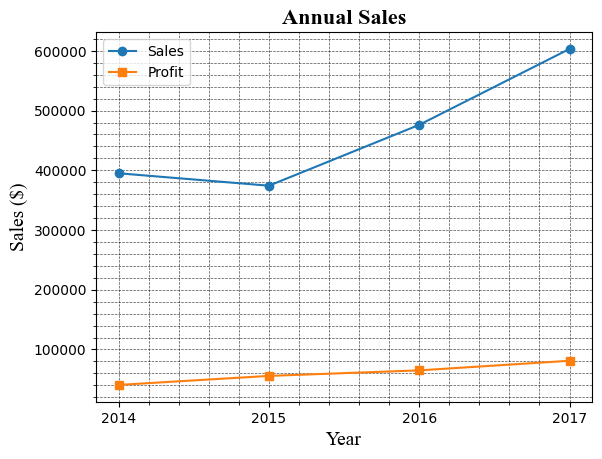
\includegraphics[keepaspectratio]{superstoreAnalysis_files/figure-pdf/cell-11-output-1.png}}

\textbf{Key Observations}

\begin{itemize}
\item
  Anual Sales

  Annual sales show a clear upward trend from 2015 to 2017, indicating
  strong business growth after a slight dip in 2015.

  The significant increase between 2016 and 2017 suggests that business
  strategies implemented during this period were highly effective in
  driving revenue.
\item
  Profit

  Profit follows a consistent upward trend, increasing each year.

  This indicates that the business is not only generating more revenue
  but is also maintaining profitability as it scale

  Although, there has been a significant gap between the anual sales
  measured to be approximately, 345k in 2014 and 522k in 2017, meaning
  the gap has increased
\end{itemize}

\textbf{Insight}

Overall the anual sales grow at a greater rate than anual profit. This
could be due to a number of factors, such as increased costs, lower
profit margins, or a shift towards lower-margin products. Further
analysis is required to identify the exact cause and improve overall
profitability.

\subsubsection{Monthly Sales}\label{monthly-sales}

\pandocbounded{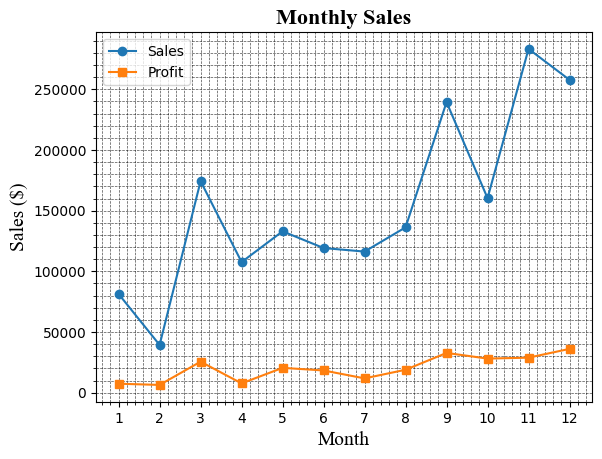
\includegraphics[keepaspectratio]{superstoreAnalysis_files/figure-pdf/cell-12-output-1.png}}

\textbf{Key Observations}

\begin{itemize}
\item
  Early-Year Dip

  Both sales and profit are significantly lower in January and February,
  with February being the lowest-performing month.

  This suggests a post-holiday slowdown, where customer spending
  typically decreases after the festive season.
\item
  Mid-Year Recovery

  From March onward, there is a sharp increase in sales, followed by
  moderate fluctuations between April and August.

  This indicates a period of stabilized business activity, where sales
  are consistent but not at peak levels.
\item
  Late-Year Surge

  A strong upward trend is observed from September through December,
  with:

  \begin{enumerate}
  \def\labelenumi{\arabic{enumi}.}
  \tightlist
  \item
    A major peak in November
  \item
    Sustained high performance in December
  \end{enumerate}

  Profit follows a similar pattern, confirming that this is the most
  valuable period for the business.
\end{itemize}

\textbf{Insight}

The business shows clear seasonal behavior:

\begin{enumerate}
\def\labelenumi{\arabic{enumi}.}
\tightlist
\item
  Weak performance at the start of the year
\item
  Strong performance toward the end of the year
\end{enumerate}

\textbf{Reccomendations}

To improve overall performance, the business should \textbf{focus on
boosting sales during the slower early months} while fully capitalizing
on the high-demand period at the end of the year.

\begin{center}\rule{0.5\linewidth}{0.5pt}\end{center}

\subsection{Regional Perfomance}\label{regional-perfomance}

\subsubsection{Overview}\label{overview}

This section analyzes sales performance across 4 regions: West, East,
Central, and South using Sales, Profit, and Profit Margin.

\subsubsection{Sales by Region}\label{sales-by-region}

\pandocbounded{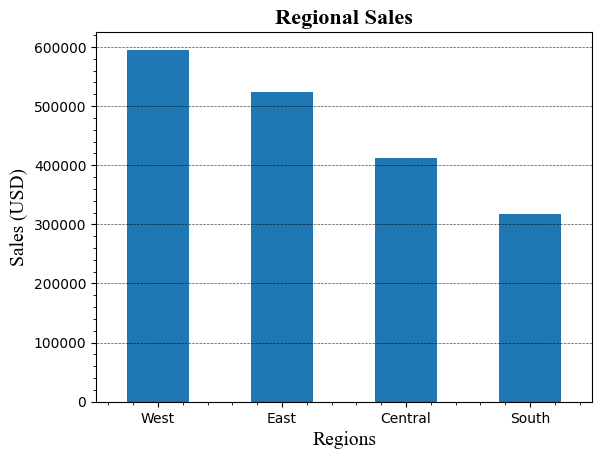
\includegraphics[keepaspectratio]{superstoreAnalysis_files/figure-pdf/cell-13-output-1.png}}

\textbf{Key Observations}

\begin{itemize}
\item
  Top Performing Region

  The West region generates the highest sales, followed closely by the
  East.

  This indicates that these regions are the \textbf{primary drivers} of
  revenue for the business.
\item
  Mid-Level Performance

  The Central region shows moderate performance, contributing a
  significant portion but still trailing behind the top regions.
\item
  Underperforming Region

  The South region records the lowest sales, generating substantially
  less revenue than all other regions.

  Compared to the West, the South generates approximately 47\% less
  revenue, highlighting a clear performance gap.
\end{itemize}

\textbf{Insight}

There is a clear imbalance in regional performance, with revenue
concentrated in the West and East.

This could be due to:

\begin{enumerate}
\def\labelenumi{\arabic{enumi}.}
\tightlist
\item
  Differences in market demand
\item
  Unequal resource allocation
\item
  Variations in marketing effectiveness
\item
  Regional economic factors
\end{enumerate}

\textbf{Recommendations}

\begin{enumerate}
\def\labelenumi{\arabic{enumi}.}
\item
  Investigate South Region Performance

  \begin{enumerate}
  \def\labelenumii{\arabic{enumii}.}
  \tightlist
  \item
    Analyze customer behavior and demand in the South
  \item
    Evaluate whether the region is under-marketed or under-supplied
  \item
    Identify barriers such as pricing, logistics, or product fit
  \end{enumerate}
\item
  Leverage High-Performing Regions

  Study strategies used in the West and East and consider implimenting
  them in the under performingregions
\item
  Optimize Resource Allocation

  Consider redistributing marketing and operational efforts Focus on
  high-growth potential regions while improving weaker ones
\end{enumerate}

\subsubsection{Profits by Regions}\label{profits-by-regions}

\pandocbounded{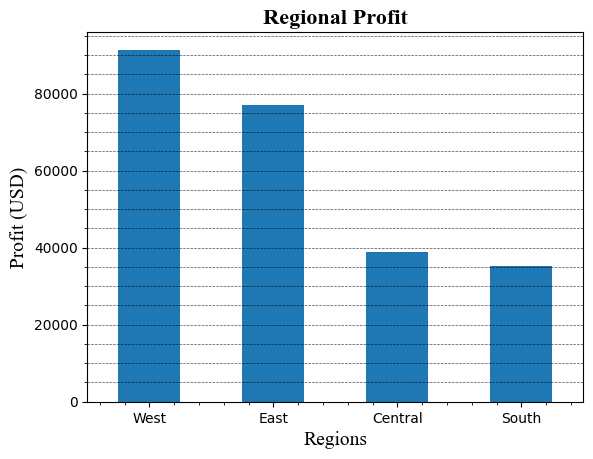
\includegraphics[keepaspectratio]{superstoreAnalysis_files/figure-pdf/cell-14-output-1.png}}

\textbf{Key Observations}

\begin{itemize}
\item
  Top Performing Regions

  The West region generates the highest profit, approximately \$91k,
  followed by the East, consistent with the trend observed in sales.

  This indicates that these regions are not only generating high revenue
  but are also maintaining strong profitability.
\item
  Central Region Concern

  The Central region generates relatively high sales (approx. 412k) but
  significantly lower profit (approx. 8.9k).

  This suggests a low return on sales, indicating potential issues such
  as:

  \begin{enumerate}
  \def\labelenumi{\arabic{enumi}.}
  \item
    High operational or shipping costs
  \item
    Heavy discounting
  \item
    Lower-margin products
  \end{enumerate}
\item
  South Region Efficiency

  Although the South region has the lowest sales (approx. 317k), its
  profit (approx. 35k) is very close to that of the Central region.

  This indicates that the South is operating with better efficiency,
  achieving similar profit levels with significantly lower sales.
\end{itemize}

\textbf{Insight:}

There is a clear difference between revenue generation and profit
efficiency across regions.

The Central region appears to be underperforming in terms of
profitability The South region, despite lower sales, is relatively more
efficient

\textbf{Recommendations:}

\begin{enumerate}
\def\labelenumi{\arabic{enumi}.}
\item
  Investigate Central Region Costs

  Analyze cost structure (logistics, discounts, operations) Identify
  areas where profit margins are being reduced Optimize pricing or
  reduce unnecessary expenses
\item
  Learn from South Region Efficiency

  Identify what is working well in the South Replicate efficient
  practices in other regions, especially Central
\item
  Strengthen High-Profit Regions

  Continue investing in West and East, as they drive both revenue and
  profit Scale successful strategies from these regions
\end{enumerate}

\subsubsection{Profit margins}\label{profit-margins}

\pandocbounded{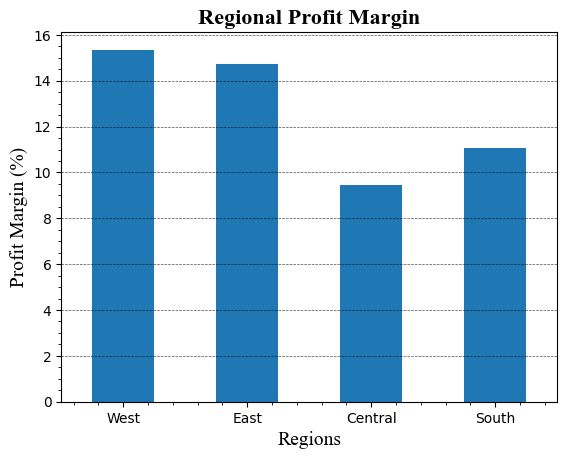
\includegraphics[keepaspectratio]{superstoreAnalysis_files/figure-pdf/cell-15-output-1.png}}

\textbf{Key Observations}

\begin{itemize}
\item
  High-Performing Regions

  The West and East regions have the highest profit margins, indicating
  strong cost control and efficient operations.
\item
  Moderate Performance

  The South region shows moderate efficiency, maintaining a reasonable
  margin despite lower overall sales.
\item
  Critical Concern: Central Region

  The Central region has the lowest profit margin (9.44\%), confirming
  earlier observations that it is underperforming in terms of
  profitability.

  This reinforces that:

  \begin{enumerate}
  \def\labelenumi{\arabic{enumi}.}
  \item
    High sales ≠ high profit
  \item
    The Central region is likely experiencing cost inefficiencies or
    aggressive discounting
  \end{enumerate}
\end{itemize}

\textbf{Insight}

Profit margin reveals the true performance of each region:

West/East: Strong revenue and strong efficiency which is why they are
best-performing regions

South: Lower revenue but decent efficiency so, it is fairly stable
Central: High revenue but poor efficiency Meaning there is prioritising
issues

\textbf{Recommendations}

\begin{enumerate}
\def\labelenumi{\arabic{enumi}.}
\item
  Fix Central Region Profitability (High Priority)

  \begin{enumerate}
  \def\labelenumii{\arabic{enumii}.}
  \tightlist
  \item
    Review products in the Central region with:

    \begin{enumerate}
    \def\labelenumiii{\arabic{enumiii}.}
    \tightlist
    \item
      Discount rates \textgreater{} 15\%
    \item
      Low profit margins
    \end{enumerate}
  \item
    Target: Increase Central region profit margin from 9.44\% → at least
    12\% within 2 quarters
  \end{enumerate}
\item
  Audit pricing strategies in Central:

  \begin{enumerate}
  \def\labelenumii{\arabic{enumii}.}
  \tightlist
  \item
    Identify products consistently sold at reduced margins
  \item
    Implement minimum margin thresholds to prevent loss-leading sales
  \end{enumerate}
\item
  Shift focus toward:

  \begin{enumerate}
  \def\labelenumii{\arabic{enumii}.}
  \tightlist
  \item
    High-margin products
  \item
    Bundled offerings instead of heavy discounts
  \item
    Reducig reliance on low-margin, high-volume items
  \end{enumerate}
\item
  Replicate High-Performing Region Strategies
\end{enumerate}

\begin{center}\rule{0.5\linewidth}{0.5pt}\end{center}

\subsection{Categories}\label{categories}

\pandocbounded{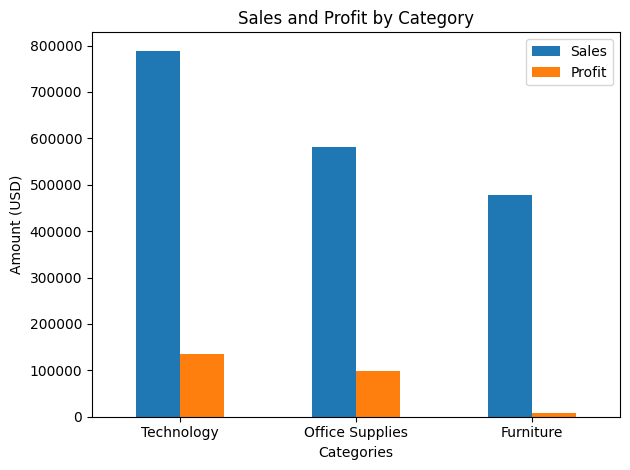
\includegraphics[keepaspectratio]{superstoreAnalysis_files/figure-pdf/cell-16-output-1.png}}

\textbf{Key Observations}

The ratio between the sales vs profit is large due to category being
broad.

\begin{itemize}
\item
  Top Performing Category: Technology

  Technology generates the highest sales and the highest profit by a
  large margin.

  This indicates:

  \begin{enumerate}
  \def\labelenumi{\arabic{enumi}.}
  \tightlist
  \item
    Strong demand
  \item
    High-margin products
  \item
    Effective pricing strategy
  \end{enumerate}
\item
  Stable Performer: Office Supplies

  Office Supplies shows solid performance in both sales and profit,
  making it a reliable contributor to overall business revenue.
\item
  Critical Issue: Furniture Category

  Furniture generates significant sales (\textasciitilde478k) but
  extremely low profit (approx. 8.9k).

  This a profit margin of roughly:

  \textasciitilde1.9\% (very low compared to other categories)

  This suggests:

  \begin{enumerate}
  \def\labelenumi{\arabic{enumi}.}
  \tightlist
  \item
    High costs (shipping, production, storage)
  \item
    Heavy discounting
  \item
    Low-margin products
  \end{enumerate}
\end{itemize}

\textbf{Insight}

Technology contributes the most to business growth and is the profit
driver. Office Supplies are the stable backbone pf the business. Lastly
Furniture is where the problem area (revenue without value)

\textbf{Recommendations}

\begin{enumerate}
\def\labelenumi{\arabic{enumi}.}
\item
  Fix Furniture Profitability (High Priority) Identify top-selling
  furniture products with low margins
\item
  Reduce Loss-Making or Low-Margin Products
\item
  Increase marketing and inventory for Technology products Expand
  product range in high-performing sub-categories
\end{enumerate}

\begin{center}\rule{0.5\linewidth}{0.5pt}\end{center}

\subsection{Top-Selling Products}\label{top-selling-products}

\pandocbounded{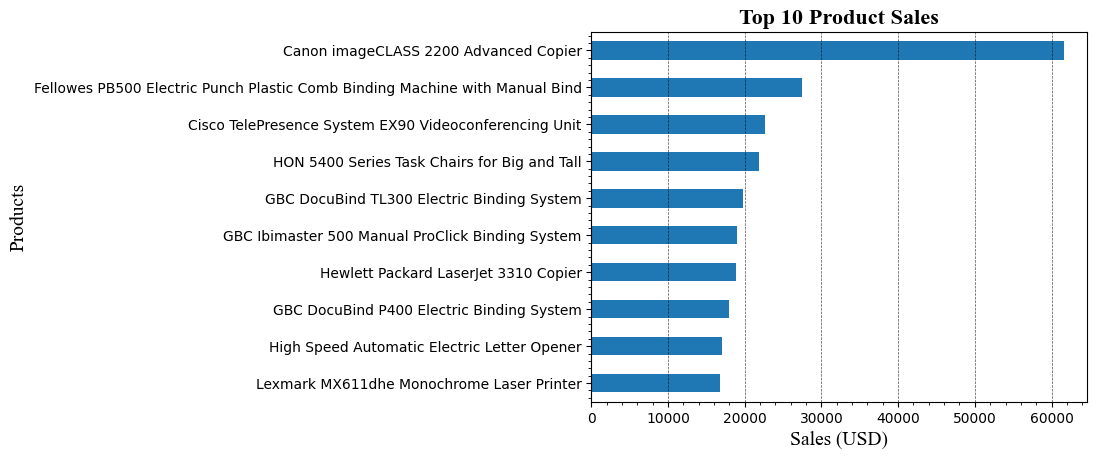
\includegraphics[keepaspectratio]{superstoreAnalysis_files/figure-pdf/cell-17-output-1.png}}

\textbf{Key Observations}

\begin{itemize}
\item
  Technology Dominance

  Many of the top products fall under the Technology category,
  reinforcing earlier findings that technology is the \textbf{primary
  revenue driver} of the business
\item
  Furniture Presence

  Products like task chairs appear among top sellers, but earlier
  analysis showed Furniture has low profit.

  This suggests furniture products may sell well, but are likely
  low-margin or high-cost
\end{itemize}

\textbf{Insight}

High-value products seem to drive revenue A strong Technology segment
for profitability

However, some top-selling products may not be highly profitable,
especially in categories like Furniture

\textbf{Recommendations}

\begin{enumerate}
\def\labelenumi{\arabic{enumi}.}
\item
  Identify which of these top-selling products: Have low or negative
  profit margins
\item
  Prioritize High-Profit Products Focus marketing and promotions on:
  Products with both high sales AND high profit
\item
  Optimize supply chain costs
\item
  Bundle high-margin + high-demand products
\item
  Invest more in Technology Category since its products are the top
  sellers
\end{enumerate}

\begin{center}\rule{0.5\linewidth}{0.5pt}\end{center}

\subsection{Segments}\label{segments}

\subsubsection{Sales}\label{sales}

\pandocbounded{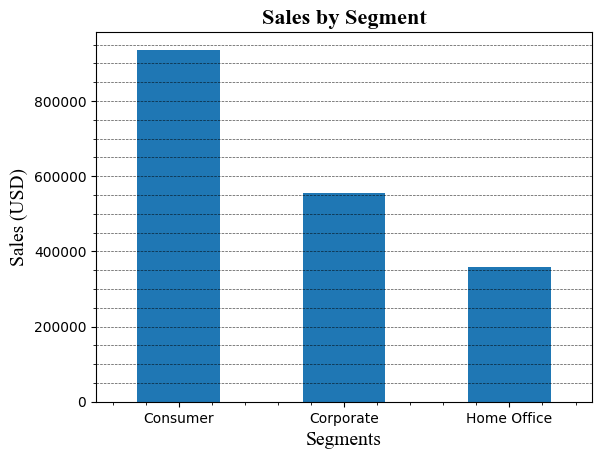
\includegraphics[keepaspectratio]{superstoreAnalysis_files/figure-pdf/cell-18-output-1.png}}

\textbf{Key Observation}

\begin{itemize}
\item
  Primary Revenue Driver

  The Consumer segment generates the highest sales compaared to the
  Corprate and Home Office segments.

  This indicates that individual customers are the main source of
  revenue for the business.
\item
  Secondary Contributor

  The Corporate segment contributes a substantial portion of sales, but
  still trails behind Consumer customers.

  This suggests steady demand from businesses, though not at the same
  scale as individual buyers.
\item
  Lowest Performing Segment

  The Home Office segment generates the lowest sales.

  This may indicate lower demand or less targeted marketing toward this
  segment
\end{itemize}

\textbf{Insight}

The business relies heavily zon the Consumer segment, making it the core
revenue engine.

However, this also introduces risk such as over-dependence on one
segment.

\textbf{Recommendations}

\begin{enumerate}
\def\labelenumi{\arabic{enumi}.}
\item
  Continue investing in Consumer Segment (Maintain Growth)

  \begin{itemize}
  \tightlist
  \item
    Marketing campaigns
  \item
    Promotions
  \item
    Product availability
  \end{itemize}

  Since this is your largest revenue driver --- protect and grow it
\item
  Expand Corporate Segment Opportunities by introducing long-term
  contracts.
\item
  Grow Home Office Segment by developing targeted campaigns for:

  \begin{enumerate}
  \def\labelenumii{\arabic{enumii}.}
  \tightlist
  \item
    Remote workers
  \item
    Small/home-based businesses
  \item
    Offer bundled office setups or affordable product packages
  \end{enumerate}
\item
  Segment-Specific Strategy

  \begin{itemize}
  \tightlist
  \item
    Avoid a using one approach for every segment. Review the statistics
    of the perfomance of each segment and strategise accordingly.
  \item
    Tailor pricing, promotions, and products for each segment
  \end{itemize}
\end{enumerate}

\subsubsection{Profit}\label{profit}

\pandocbounded{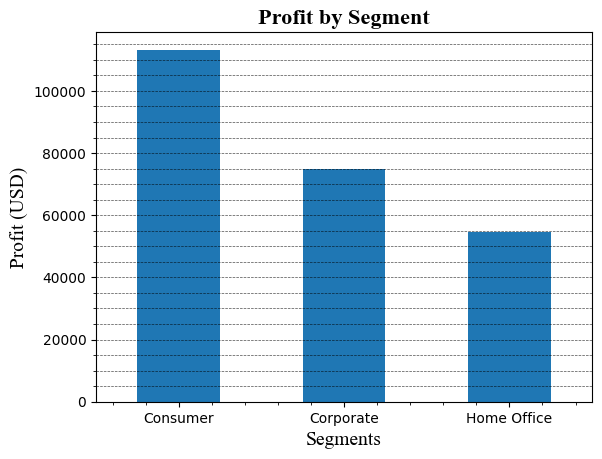
\includegraphics[keepaspectratio]{superstoreAnalysis_files/figure-pdf/cell-19-output-1.png}}

\textbf{key Observations}

\begin{itemize}
\item
  Consistency

  The profits remain consistent with the sale. Although the Home Office
  segment has the lowest sales, it still generates a notable level of
  profit (approximately 54k) suggesting potentially higher margins
  compared to its size
\end{itemize}

\textbf{Insight}

When comparing sales vs profit across segments:

Consumer: - Have a high sales and high profit making them the
\textbf{core growth engine} Corporate: - Have moderate sales and profit
making Corporate the \textbf{stable contributor} Home Office: - Have the
lowest sales but decent profit making them have \textbf{unnoticed
potential}

This tells that the business is not just driven by volume (Consumer),
but also has efficient smaller segments (Home Office) that can be
expanded.

\textbf{Recommendations}

\begin{enumerate}
\def\labelenumi{\arabic{enumi}.}
\item
  Continue Scaling Consumer Segment by maintaining strong marketing and
  product availability
\item
  Strengthen Corporate Relatiionships by utilising the long term
  contract metioned previously
\item
  \textbf{Expand Home Office Segment:}

  \begin{itemize}
  \item
    Target, remote workers, freelancers, small businesses, etc and
    capitalize on them
  \item
    Offer affordable starter kits to help attract clients of the Home
    Office Segment, which has the highest potential
  \item
    Increase sales while maintaining current efficiency
  \item
    Since technology has the highest sales, the business should consider
    investing more of it into this segment
  \end{itemize}
\item
  Segment Profitability Strategy -Analyze profit margins per segment;
  which segment converts revenue into profit most efficiently
\end{enumerate}

\subsubsection{Profit Margin}\label{profit-margin}

\pandocbounded{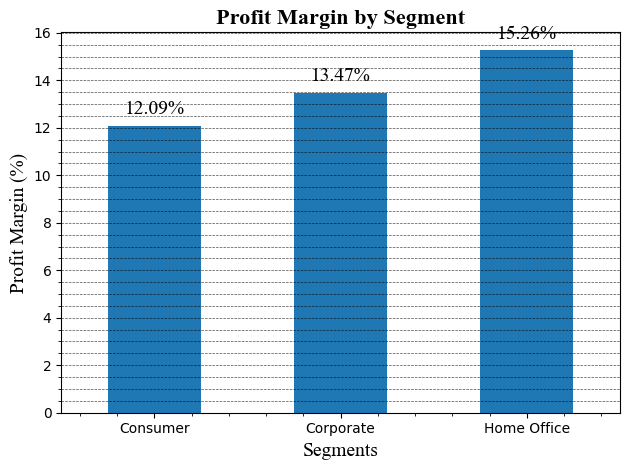
\includegraphics[keepaspectratio]{superstoreAnalysis_files/figure-pdf/cell-20-output-1.png}}

\begin{center}\rule{0.5\linewidth}{0.5pt}\end{center}

\subsection{KPIs used}\label{kpis-used}

The following key performance indicators (KPIs) were used to evaluate
business performance:

\textbf{Total Sales}

Measures overall revenue generated across different dimensions (time,
region, category, and segment).

\textbf{Total Profit}

Indicates the net earnings after costs, used to assess overall
profitability. Profit Margin (\%)

Calculated as (Profit / Sales × 100), this metric evaluates how
efficiently the business converts revenue into profit.

\textbf{Sales Growth (Annual Trend)}

Tracks changes in revenue over time to identify business growth
patterns. Seasonal Trends (Monthly Sales \& Profit) Identifies
fluctuations in performance throughout the year.

\textbf{Regional Performance}

Compares sales and profit across regions to detect geographical
strengths and weaknesses. Category \& Product Performance Evaluates
which product categories and individual products drive revenue and
profit.

\textbf{Customer Segment Performance}

Analyzes contribution from different customer groups (Consumer,
Corporate, Home Office). Compared the rates between the sales an profits
of each segment by calculating: (each segment profit / each segment
sale) and ploting that

\begin{center}\rule{0.5\linewidth}{0.5pt}\end{center}

\subsection{\texorpdfstring{\textbf{Key
Takeaways}}{Key Takeaways}}\label{key-takeaways}

The analysis reveals that the business is experiencing \textbf{steady
growth in both sales and profit}, although profit is increasing at a
slower rate, indicating a \textbf{decline in efficiency}. There is a
clear \textbf{seasonal pattern}, with performance peaking toward the end
of the year and dipping in the early months. Regionally, \textbf{the
West and East drive the majority of revenue}, while the \textbf{Central
region underperforms in profitability}, highlighting inefficiencies.
From a product perspective, \textbf{Technology is the strongest
category}, whereas \textbf{Furniture generates high sales but very low
profit}, making it a key concern. The \textbf{Consumer segment is the
primary revenue and profit driver}, though opportunities exist to expand
the \textbf{Home Office segment} and leverage the \textbf{efficiency
observed in the South region}. Overall, the business should
\textbf{focus on improving low-margin areas while scaling its
high-performing segments and categories}.




\end{document}
